\setlength{\columnsep}{3pt}
\begin{flushleft}
\bigskip
\bigskip

\textbf{The rules in /etc/rsyslog.conf} defines what files the logs are redirected according to \textbf{facility \& severity} using below syntax:

\begin{tcolorbox}[breakable,notitle,boxrule=-0pt,colback=pink,colframe=pink]
	\color{black}
	\fontdimen2\font=1em
	Syntax: facility.severity      logfile-name
	\fontdimen2\font=4pt
\end{tcolorbox}

Eg:
\begin{figure}[h!]
	\centering
	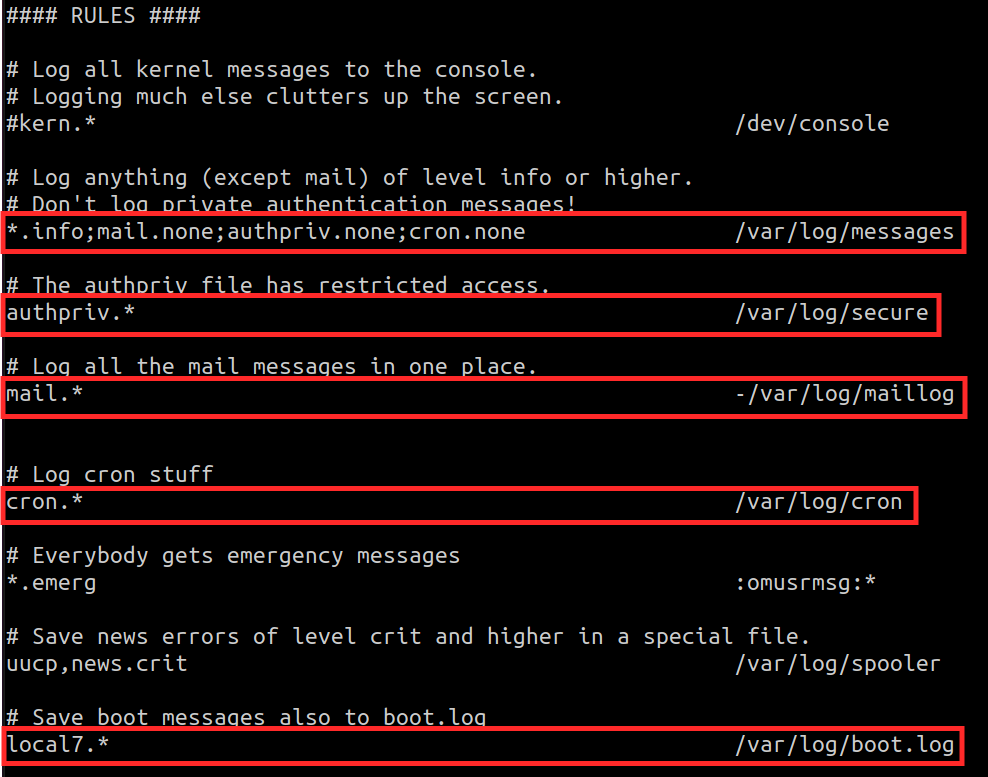
\includegraphics[scale=0.4]{content/chapter16/images/rsyslog.png}
	\caption{Facility \& severity setting in /etc/rsyslog.conf}
	\label{fig:s1everity}
\end{figure}

Let's see more on \textbf{facility \& severity}.

\newpage

\textbf{Facility levels}:
The facility represents the machine process that created the syslog event. Below are the available facility levels:
\begin{figure}[h!]
	\centering
	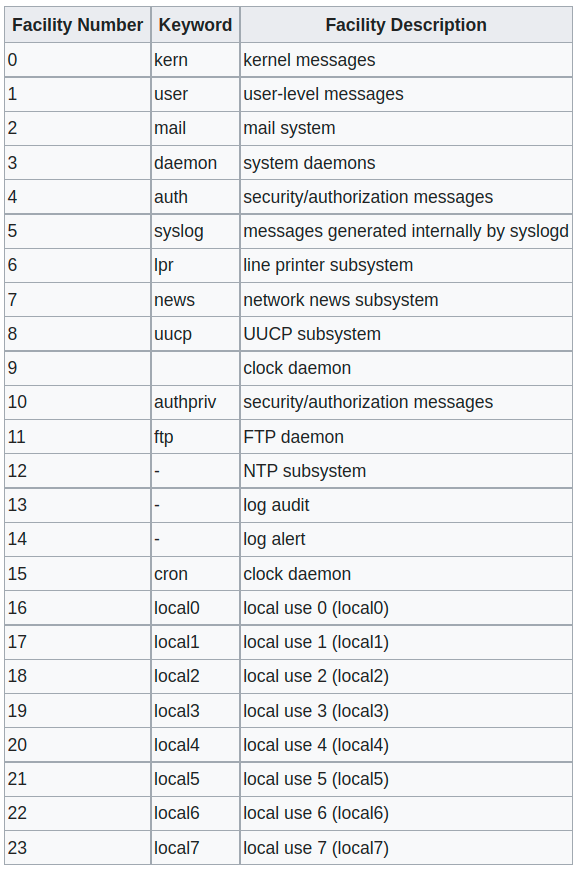
\includegraphics[scale=0.5]{content/chapter16/images/facility.png}
	\caption{Log facility}
	\label{fig:facility}
\end{figure}

\newpage

\textbf{Severity also known as Priority}:
The severity level describes the severity of the log in question.
\begin{figure}[h!]
	\centering
	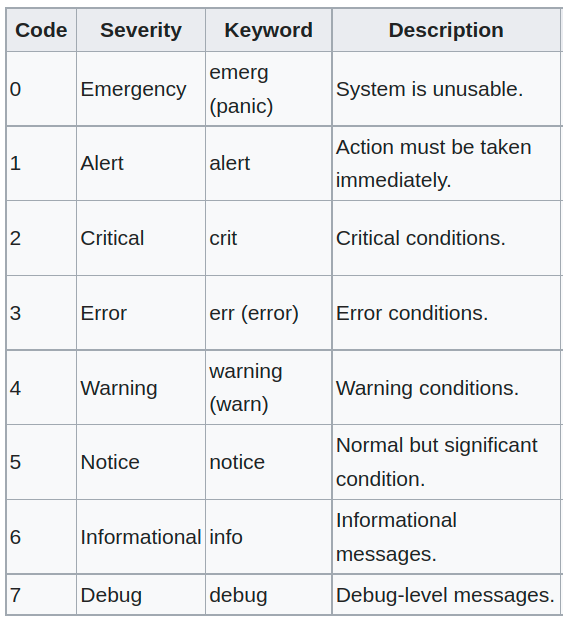
\includegraphics[scale=0.65]{content/chapter16/images/priority.png}
	\caption{Log Severity}
	\label{fig:severity}
\end{figure}




\end{flushleft}
\newpage


